\documentclass[11pt, twocolumn]{article}
\usepackage[utf8]{inputenc}

\usepackage[usenames,dvipsnames]{color} % Required for custom colors

\usepackage{graphicx} % Required to insert images
\usepackage{caption}
\usepackage{subcaption}

\usepackage{listings} % Required for insertion of code
\lstloadlanguages{[ISO]C++, HTML, PHP, MATLAB,TeX, Python}

\usepackage[x11names, rgb, html]{xcolor}

% Solarized colors
\definecolor{sbase03}{HTML}{002B36}
\definecolor{sbase02}{HTML}{073642}
\definecolor{sbase01}{HTML}{586E75}
\definecolor{sbase00}{HTML}{657B83}
\definecolor{sbase0}{HTML}{839496}
\definecolor{sbase1}{HTML}{93A1A1}
\definecolor{sbase2}{HTML}{EEE8D5}
\definecolor{sbase3}{HTML}{FDF6E3}
\definecolor{syellow}{HTML}{B58900}
\definecolor{sorange}{HTML}{CB4B16}
\definecolor{sred}{HTML}{DC322F}
\definecolor{smagenta}{HTML}{D33682}
\definecolor{sviolet}{HTML}{6C71C4}
\definecolor{sblue}{HTML}{268BD2}
\definecolor{scyan}{HTML}{2AA198}
\definecolor{sgreen}{HTML}{859900}

\lstset{
    % How/what to match
    sensitive=true,
    % Border (above and below)
    frame=lines,
    % Extra margin on line (align with paragraph)
    xleftmargin=\parindent,
    % Put extra space under caption
    belowcaptionskip=1\baselineskip,
    % Colors
    backgroundcolor=\color{sbase3},
    basicstyle=\color{sbase00}\ttfamily,
    keywordstyle=\color{scyan},
    commentstyle=\color{sbase1},
    stringstyle=\color{sblue},
    numberstyle=\color{sviolet},
    identifierstyle=\color{sbase00},
    % Break long lines into multiple lines?
    breaklines=true,
    % Show a character for spaces?
    showstringspaces=false,
    tabsize=2
}

\usepackage{courier} % Required for the courier font
\usepackage{float}

\usepackage{multicol}
\usepackage{amssymb}
\usepackage{amsmath}

\usepackage{natbib}
\bibliographystyle{plainnat}

%\title{Numerical simulation and modeling to promote expert-like behaviour and competence in applied physics among students}
\title{Gamification of modeling to promote expert-like behaviour and competence in applied physics among university students}
\author{Daniel Kastinen}
\date{February 2021}

% Margins
\topmargin=-0.9in
%\evensidemargin=0in
%\oddsidemargin=0in
\textwidth=6.5in
\textheight=9.0in
%\headsep=0.25in

\begin{document}

\maketitle

\section{Introduction}

Traditional university level education in introductory physics does not contain a significant amount of interactive engagement as it is mostly based on passive lectures. Research shows that interactive engagement promotes learning by a significant amount \citep{hake1998interactive, prince2004does}. Traditional education is however not completely void of interactive engagement as laboratory work is a common part of most introductory physics courses. However, many studies show that simply implementing laboratory work in a course without the proper direction and iterative development does not bring that much benefit \citep{holmes2018introductory, redish2004teaching}. Using laboratory work specifically tailored for certain teaching purposes and learning outcomes can greatly benefit the learning of students \citep{redish2004teaching}. With the swift development of computers both in computing power and hardware cost laboratory work is no longer restricted to physical experiments but can also consist of simulations. Recently a slew of e.g. online physics simulations have been developed to be used in interactive engagement oriented laboratory work \citep{zhou2018websites}. At the same time, it is being discovered what works and what does not when it comes to the use of physics simulations in education \citep{wieman2008oersted}. Laboratory work such as discussed above usually entails group work. It has also been shown that including a certain amount of cooperative grouping and cooperative learning, i.e group-work, can be highly beneficial to learning outcomes if done correctly \citep{heller1992teachinga}.

However, learning and knowledge acquisition is not all there is to becoming an expert in a subject. One must also adopt certain habits and behavioural patterns to become like an expert. This was studied in detail by \citet{adams2006new} where it was shown that students are not adopting expert-like attitudes and behaviour. Surprisingly, is that it was shown that students know very well what expert-like attitudes and behaviours are. They simply do not adopt them themselves. The reason for this can only be speculated about but a reasonable proposition is simply that students have not experienced situation's where expert-like attitudes and behaviours are required or justified. These situations usually comes to pass during doctorate studies and other research activities. When one realizes the need for the expert-like attitudes and behaviours in a situation they are much more easily adopted as their worth is internally affirmed. This hypotheses is supported by \citet{kapon2016doing} where a research-like situation was created in university level education and significant improvements in attitudes and behaviour was measured. In \citet{kapon2016doing}, the research-like situation created a zone of proximal development, where the problem was slightly above the competence level of the student but guidance was minimal to emulate research. The lack of guidance and need for a deeper understanding to complete the task facilitated learning and behavioural change, different to traditional teaching. However, as is also the main criticism of such methods \citep{hner2006minimal}, the project was very time consuming with compared to the small amounts of assimilated knowledge. 

The current generation of students have grown up in a society where games are readily available and plentiful. Many students today can sit down in front of a new digital game and figure out the mechanics of that game world with any instruction in only a few minutes to hours. It is reasonable to assume that this ability comes from a constant exposure to digital games. However, the methodology of discovering the rules of a game world and physics research is practically the same but the latter being much more formalized. In fact, e.g. the additional enjoyment of a well designed game has made gamification a new and exiting area of research \citep{dicheva2015gamification}. 

As was shown in \citet{redish2004teaching}, it is possible to create module like teaching activities that are tailored to achieve certain goals, that are simply slightly modified to the course where they are implemented. Following the design methodology of \citet{redish2004teaching} and \citet{heller1992teachingb}, we have created a small module of physics simulation laboratory work that specifically promotes both expert like behaviour by invoking the zone of proximal development, creating a situation that cannot be overcome without expert-like attitudes and behaviours, and teaches applied physics skills. As opposed to traditional research like elements in education, this module is accelerated by gamification in order to tap into the existing behaviour of exploration and discovery and by cooperative learning by performing the module in groups. Depending on the time available for the module, the physics to be simulated can be tailored to the needs of the course and education as a whole. Either the physics is built on existing knowledge by the students, shortening the time needed, or it is used to introduce practically a recently covered subject, requiring more time for the students to get familiar with the rules of the game. The equipment needed is a single computer per group, thus allowing this module to be highly flexible and used in almost any setting where a stronger presence of these learning goals are needed.

\section{Education Component}

\subsection{Intended Learning Outcomes}

The intended learning outcomes of this module are

\begin{itemize}
    \item[I] Improvement in expert-like attitude
    \item[II] Functional knowledge of the physics to be simulated
    \item[III] General physics modeling skills
    \item[IV] Rudimentary data analysis skills
    \item[V] Cooperation skills in research-like work
    \item[VI] New perspective on what is "current physics"
\end{itemize}

\subsection{Prerequisite Knowledge}

Before attending this module the students should have at least

\begin{itemize}
    \item Experienced some amount of scripting or programming
    \item Have had a broad overview of the simulated physics (there should be some unknown that need to be discovered)
\end{itemize}

\subsection{Course Context}

Based on the prerequisite knowledge and intended learning outcomes, it is recommended that this module take place somewhere between the end of the first year of Bachelor studies and prior to the last year of a Masters studies, i.e. somewhere between year 1-4 of University studies. The breath of possible courses is due to highly variable difficulty of the laboratory work. If more components of the physics to be modeled by the students are unknown, it will become significantly harder to discovery the correct model, rather then e.g. a single unknown component. For example, if the module is placed in a course at the end of the first year of Bachelor studies and we can assume this physics courses contain knowledge on Newtonian gravity. Then a good compromise to make is to make the physics inside the game Newtonian gravity, give the students the masses and positions of the perturbing object(s) in the game, but have the gravitational constant be different than in real life. It now quickly becomes apparent to the students that the shape of implemented models are correct but the scaling is wrong and they need to analyse the games data output to discover the new coefficient in order to beat the level. This implementation leans more towards learning outcomes (I) and (IV-VI) than (II-III). 

Depending on the extent of the module, anything between 1-4 ECTS is recommended for the laboratory work.

As was mentioned, the physics can be adapted to the course in question. We will below provide some initial suggestions:

\begin{itemize}
    \item Electromagnetism course:\newline
    Objects have positive and negative charge, constant magnetic field perpendicular to the screen, Lorenz force governs the player, possible challenge is to find the magnetic field strength and charges of the objects in the players path / the charge of the player itself.
    \item Introductory mechanics course:\newline
    The player experiences friction with the game surface where the friction coefficient is unknown, the kinetic friction coefficient might also change depending on region in the level and there might be a constant force to simulate that of a tilted plane.
    \item Introductory physics course:\newline
    Physics inside the game is Newtonian gravity, position and masses of perturbing objects are known but gravitational constant is different. Alternatively, the constant is known but the level is designed in such a way that Hohmann transfer orbits are needed to reach the goal.
    \item Quantum mechanics course:\newline
    An obstacle in the game can be "quantum tunneled" trough (lets propose a high probability, say >50\%). Once the effect is discovered the students need to analytically solve for the energy needed to tunnel trough with high enough probability for it to be profitable due to limited attempts in the game and figure out if they can reach this energy in the game.
\end{itemize}

Of course the above are only a fraction of the possible implementations available, it is up to the course examiner to decide on the most appropriate game content that matches with the course contents and intended learning outcomes.

\subsection{Material}

All the needed material for the game is available openly at this Github repository: \texttt{https://github.com/danielk333/TSDR}. This code should be forked and tailored to the course in question. The tailoring requires basic knowledge of Python 3 programming. Additionally, there is game instructions in the repository but ideally a specific laboratory instruction document should be constructed for the specific course depending on how the module is implemented.

\subsection{Teaching and Learning Plan}

\begin{figure*}
    \centering
    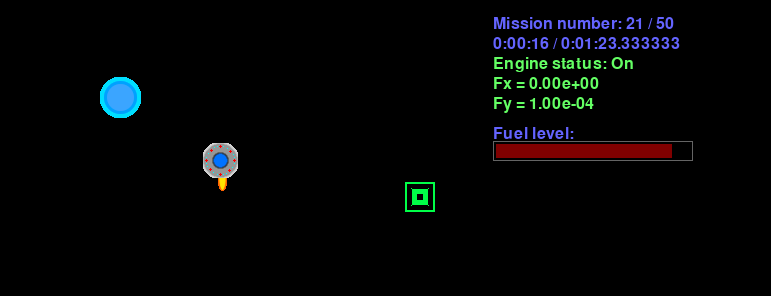
\includegraphics[width=0.9\hsize]{game_frame.png}
    \caption{A frame of the game experiment mode in action.}
    \label{fig:game_frame}
\end{figure*}


The module itself can be divided into three segments:
\begin{enumerate}
    \item Introductory session:\newline
    Possible pre-test, introduction to the exercise, division into groups, hand out of information, checking that everyone can run the game and understands the task, initial questions from the students.
    \item Laboratory work sessions:\newline
    At least first session supervised, supervision on reaming sessions depend on the course context. Students play the game, model the physics and perform the necessary data analysis. Many questions are predicted to arise not in the very beginning of exploration but in the middle, where the goals have become clear (e.g. find the gravitational constant) but the path there is not (fit the implemented model with the force data output from the game using e.g. lest squares minimization with the gravitational constant as a free parameter). Each sessions should end with a class discussion on the thoughts regarding what the goals are to beat the game and how to reach them, and the relationship between the work performed by the students and real life research and work. All groups should keep detailed logbooks on their thinking and work: what experiments are they running, what information do they look for, what problems do they experience, what are their solutions, ect. This together with valid solution code is the examining moment for the module.
    \item Solution reviews:\newline
    All group solutions to both the force model implemented and the thrust program implemented to reach the goal are presented by the group in front of the class. The solution is visualized by prepared software that only the examiner has and the solutions are briefly discussed in the class. Possible post-test.
\end{enumerate}

\subsection{Game}


\begin{figure*}
    \centering
    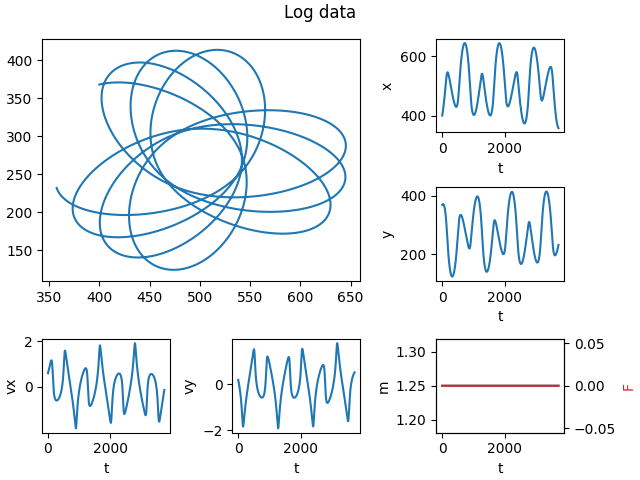
\includegraphics[width=0.9\hsize]{game_log.png}
    \caption{The quick-look plot of the log output by the game of a experiment using no thruster. The log is CSV formatted and easily loaded into any analysis software of choice.}
    \label{fig:game_log}
\end{figure*}

The game is about exploring an new realm with unknown physics using an autonomous probe, the goal being to move on to the next domain. The player has the possibility to either launch an automated probe with a specific thruster program into the new realm, generating a logfile of output data as measured by the probe, or to simulate the trajectory of the next probe using a model of the physics in this new realm. There is only a limited amount of launch attempts so one cannot be wasteful and just brute force the thruster program to find the solution. Much like spacecraft today, simulation prior to excursion is extremely useful when one can only afford to try something once or twice. Modeling the physics to match what happend in the first probe launch and then writing the thruster program is playing the game.

To test the game in the the current state of the base repository
\begin{enumerate}
    \item Clone the repository\footnote{\label{link}\texttt{https://github.com/danielk333/TSDR}}
    \item Run \texttt{pip install -r requirement.txt}
    \item Run \texttt{python run.py} to display the initial help needed to play.
    \item The save game data is in the \texttt{game/data/save\_data.npy}, to restart the game: delete this file.
\end{enumerate}

To install on student computers
\begin{enumerate}
\item Clone the repository\footnotemark[\ref{link}]
\item Run \texttt{pip install -r requirement.txt}
\item run \texttt{python compile.py "path/to/game"}. The path should NOT be inside the repository. 
\item Delete the repository.
\item Run the game with \texttt{python run.py [args]} from the \texttt{path/to/game} directory. All data output from the game will now be stored in this directory.
\end{enumerate}

After the above steps, there should be a compiled game package in the given path, together with a \texttt{run.py} where the student input is stored. When this file is run with \texttt{python run.py} help text is displayed with available game commands. When the game is setup in an actual classroom, there should also be a prepared document with instructions in this folder specific for the course in question together with other possible needed information, e.g. a \texttt{numpy} cheat-sheet.

When deployed in a course, an additional layer of encryption should probably be put on the game configuration and the pass-codes file so that the game decrypts the files to read the data from them. This prevents to students from "cheating". This is currently not implemented by default so the files are visible in plain-text.

The game has 3 major modes:
\begin{itemize}
    \item exp [realm number]: Experiment mode, launches an experiment into the new realm. The probe records all data it can, including its position, velocity, mass and thrust generated. The goal is to reach the next portal, otherwise the probe will be stranded and lost, although we always get the logfiles back.
    \item log [log number]: Log quick-look mode, plots the logfile from an experiment to view. This data will need to be more carefully analyzed but a first look is always good to have.
    \item sim [realm number]: Perform a simulation of an experiment. The simulation uses the model given by the player to predict the trajectory of the probe. If the physics model is correct, this simulation can be used to figure out how to create the automated thruster program that will get us to the goal!
    \item bank [passcode]: Redeem a passcode to receive more attempted experiments, i.e. more probe launches.
\end{itemize}

The main reason for the "bank" mode is the possible permanent loss state of the game. Some students might simply try to spam solutions and then not have more attempts to complete the exercise. The limitation on probe launch attempts is needed as it forces the students to model the physics so the next launch is known to succeed. If they need more chances, a system to earn passcodes can be put in place. One possible method is to have a set of analytic problems related to the tasks in the game, e.g. curve fitting, derivation of Hohmann transfer orbits, problems with the Lorenz force, ect. Handing in solutions to these problems earn them passcodes.

A typical game round might be
\begin{enumerate}
\item Clear the thruster control system so that it is completely turned off.
\item Launch an experiment with \texttt{python run.py exp}.
\item Watch the outcome, get familiar with the environment.
\item Plot the log with \texttt{python run.py log}, look at the forces that affect the probe.
\item Load the logfile into some analysis program written by the player, create an analytic model of the force, write it in the \texttt{def force(...):} function in \texttt{run.py}.
\item Run a simulation with the new force model using \texttt{python run.py sim}. If the trajectory looks like the logfile, you have discovered and modeled the physics!
\item Write a parameter controlled thruster program, run a simulation again using \texttt{python run.py sim}, but this time tune the parameters using the TK interface.
\item Find a thruster program that gets to the goal, put those parameters into the \texttt{get\_control\_params} function.
\item Launch a new experiment with \texttt{python run.py exp} and cross your fingers! Hopefully you win!
\end{enumerate}

As of writing, the \texttt{run.py} file that students initially are faced with is listed in Figure~\ref{fig:run}. An example screenshot of the game running is illustrated in Figure~\ref{fig:game_frame}. An example of the output from the games log quick-look function is illustrated in Figure~\ref{fig:game_log} and finally, a screenshot of the simulation game mode is shown in Figure~\ref{fig:game_simulation}. Here the defined parameters of the thurster algorithm is available for quick editing to find the correct parameters needed to win the game, given that the physics have been correctly modeled.

\begin{figure*}
    \centering
\begin{lstlisting}[language=Python]
import sys
import numpy as np

from game import run


def get_control_params():
    '''These are the parameters that control the "thrust" algorithm. They will appear as float variables in the simulation.'''
    params = dict(
        t_start = 1e3,
        force_y = 0,
        force_x = 0,
    )
    return params


def thrust(pos, vel, t, m_wet, **params):
    '''Thruster controller: takes in ship position, velocity, time and the current fuel mass.
    Returns the vector force that the thrust should generate for that time.

    In the keyword arguments "params" are the parameters to control the algorithm.
    When running the actual experiment the parameters used will be fetched from "get_control_params".
    When simulating a mission, the parameters can be changed on the fly since it is a simulation.
    '''
    if t > params['t_start']:
        return np.array([params['force_x'],params['force_y']])
    else:
        return np.array([0.0,0.0])


def force(pos, vel, t, m):
    '''Model of the physics to be used in the simulation, a function of position, velocity, time and mass of the object experiencing the force.'''
    return np.array([0.0,0.0])

if __name__=='__main__':
    run(get_control_params, thrust, force, sys.argv)
\end{lstlisting}
    \caption{The entry point \texttt{run.py} for the game. This is where students enter their thruster algorithm and model the force in the game.}
    \label{fig:run}
\end{figure*}



\begin{figure*}
    \centering
    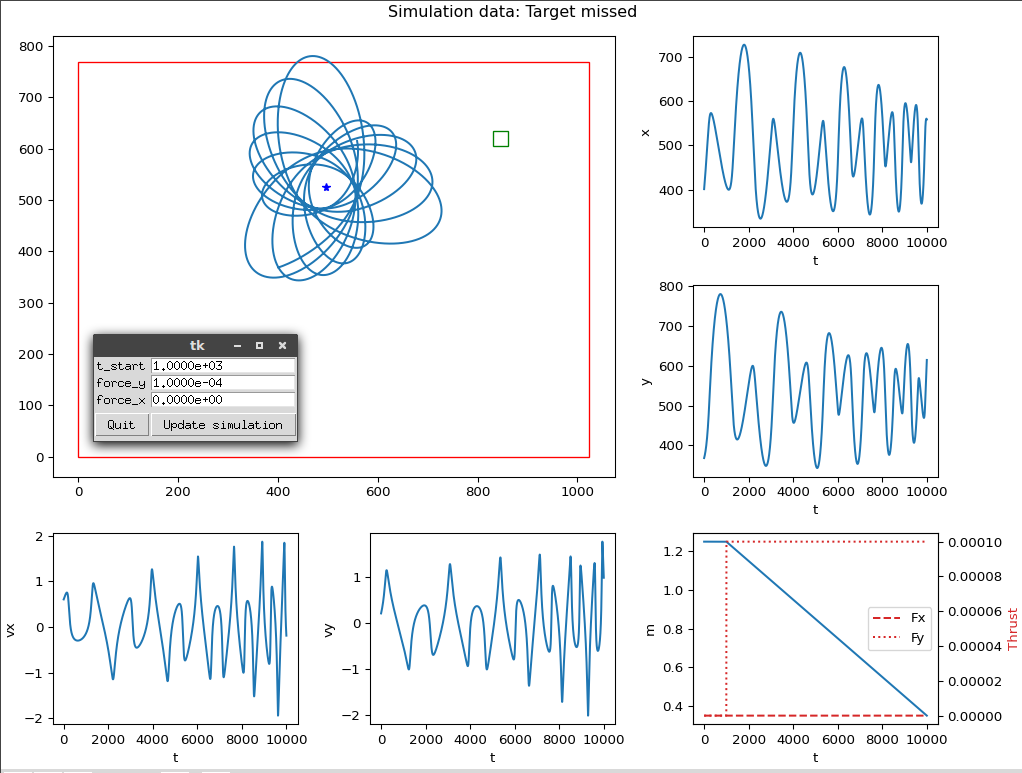
\includegraphics[width=0.9\hsize]{game_simulation.png}
    \caption{A screenshot of the simulation component of the game. This uses a slightly correct force model and the standard thruster program as also described in \ref{fig:run}. All parameters listed are available trough the input-panel so that fine tuning of the algorithm parameters in preparation for the actual experiment probe launch.}
    \label{fig:game_simulation}
\end{figure*}

\subsection{Assessment}

The assessment of the students will employ mostly formative authentic assessment \citep{lombardi2008making, lyon2011problem} on the form of

\begin{itemize}
    \item Small written summary (less then 1 page) of the modeling implementation and thruster control (summative traditional assessment)
    \item Continues logbook kept by groups on methodology of performing the laboratory work, from start to finish (formative authentic assessment)
    \item End-of-session summary on ideas and progress from each group, short class discussion (formative authentic assessment)
\end{itemize}

\section{Evaluation}

\subsection{Pre- and post-test}

As all intended learning outcomes besides (I) should be tested by the overall course examination, only the change in expert-like attitudes of the student remain to be tested. For this pourpuse we propose to use CLASS version 3 \citep{adams2006new} as this was also used to initially determine the expert like attitudes of students. Version 3 has six item that are not scored as they were not productive in their current form, these questions should ideally be changed to better sample the intended learning outcomes of the module that are not already covered by the overall course testing. An example of this might be the change in viewpoint on "current physics" or the change in attitude towards applied physics and modeling.

\subsection{Interviews}

To facilitate an iterative approach to module development according to \citet[Ch.6][]{redish2004teaching} a small sample of interviews with students should be conducted after completion of each course.


%----------------------------------------------------------------------------------------
\newpage

\addcontentsline{toc}{section}{References}
\bibliography{cite}


\end{document}

